\chapter{Arquitectura del sistema}
\section{Diseño general del sistema}

Descripción en prosa del diseño del sistema. Resalte cualquier detalle que considere de importancia para la comprensión del diseño.

\subsection{Diagrama de clases}
Añada una imagen con el diagrama de clases del sistema,  preferiblemente desarrollado en DIA. Introdúzcala con un párrafo breve que enlace el diagrama con la descripción en prosa del encabezado de sección. Se recomienda que el diagrama se diseñe de forma que calce bien en una página vertical, de forma que se facilite su lectura. Recuerde hacer referencia a su diagrama de clases usando la referencia correcta. Por ejemplo, en la Figura \ref{DiagramaClases} se encuentra el diagrama de clases.
\begin{figure}[H]
  \centering
    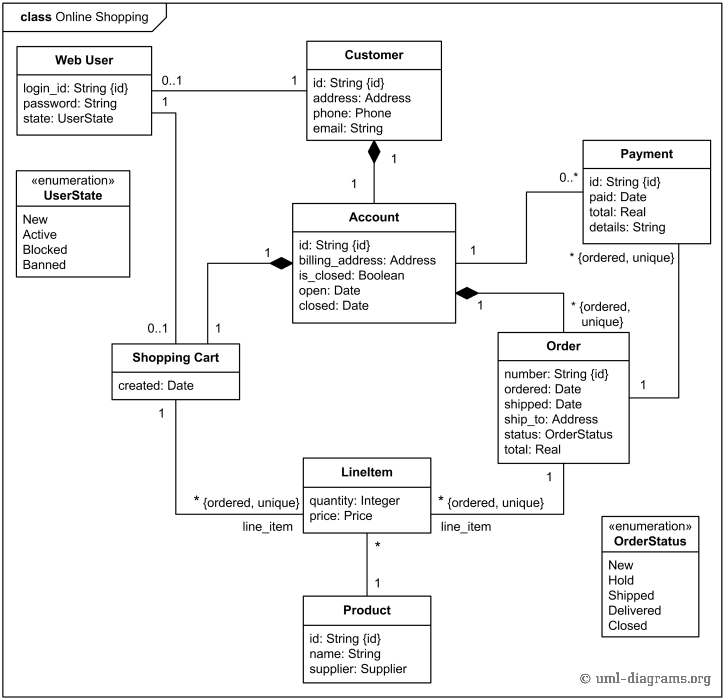
\includegraphics[ width=15cm]{project/images/class-example-online-shopping-domain.png}
  \caption{\textbf{IMAGE CAPTION}}
  \label{DiagramaClases}
\end{figure}

\subsection{Estrategias de diseño}
Describa en esta sección la aplicación de patrones de diseño identificados para su sistema. Incluya en la descripción los problemas detectados que se resolvieron por medio de la implementación del patrón. Adicionalmente describa la forma en que se adaptaron los patrones para que funcionaran correctamente con su sistema.

